\section{Zielsetzung}
\label{sec:Zielsetzung}
In diesem Versuch wird die Maximalenergie eines $\beta$-Strahlers bestimmt und das exponentielle Absorbtionsgesetz für $\gamma$-Strahlung verifiziert. Außerdem sollen noch die Absorbtionskoeffizienten für verschiedene Materialien bestimmt werden.

\section{Theoretische Grundlage}
\label{sec:Theorie}
Die Photonen der $\gamma$-Strahlung und die Elektronen der $\beta$-Strahlung wechselwirken nicht nur mit Materie, wenn die Teilchen der Strahlung direkt auf ein Elektron oder Atomkern der Materie treffen, sondern es treten zahlreiche weitere Wechselwirkungen auf. Da Materie zum großen Teil aus Freiraum besteht, wird ein Wirkungsquerschnitt $\sigma$ definiert. Allerdings ist der Wirkungsquerschnitt keine geometrisch messbare Größe, sondern eine Wahrscheinlichkeit mit der die Teilchen wechselwirken. Die Anzahl der Wechselwirkungen sind trotzdem von der Dicke $D$ des Absorbers abhängig, als Absorber wird hier das absorbierende Material bezeichnet. Für die $\gamma$-Strahlung gilt ein exponentieller Abfall der Strahlungsintensität:
\begin{equation}
	N(D) = N_0 \cdot e^{-n\,\sigma\,D} \ .
	\label{eqn:N}
\end{equation}
Dabei entspricht $N(D)$ der Impulszahl, $n$ ist die Teilchenzahl pro Volumen des Absorbers. Aus $n$ und $\sigma$ wird der Absorbtionskoeffizient $\mu = n \cdot \sigma$ definiert. Die Teilchenzahl $n$ berechnet sich nach
\begin{equation}
	n = \frac{z\,N_\text{A}}{V_\text{mol}} = \frac{z\,N_\text{A}\,\rho}{M} \ ,
	\label{eqn:n}
\end{equation}
mit der Avogadro-Konstante $N_\text{A}$, der Ordnungszahl $z$, sowie dem Molekulargewicht $M$, dem Molvolumen $V_\text{mol}$ und der Dichte $\rho$.


\subsection{Eigenschaften von \texorpdfstring{$\gamma$}{}-Strahlung}
$\gamma$-Strahlung entsteht, wenn ein angeregter Atomkern mindestens ein Energieniveau nach unten fällt. Die Energieniveaus in einem Atom besitzten diskrete Zustände, daraus ergibt sich, dass die $\gamma$-Strahlung ein diskretes Linienspektrum hat. Da die Strahlung aus Photonen besteht, breitet sie sich mit Lichtgeschwindigkeit aus und weist die typischen Eigenschaften einer elektromagnetischen Welle, wie etwa Interferenz, auf. \\
Die $\gamma$-Strahlung wird durch unterschiedliche Effekte von der Materie absorbiert. Diese Effekte sind in der nachfolgenden Abbildung (Abb. \eqref{fig:Wechselwirkungen}) aufgelistet.

\begin{figure}[H]
	\centering
	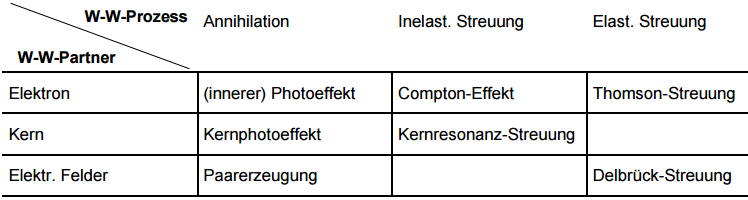
\includegraphics[height=4cm]{picture/Wechselwirkungen.PNG}
	\caption{Die Wechselwirkungen der $\gamma$-Quanten. \cite[4]{sample}}
	\label{fig:Wechselwirkungen}
\end{figure}

Allerdings treten im wesentlichen nur die Paarbildung, der Photo- und der Compton-Effekt auf. Auf diese drei Wechselwirkungen wird im folgenden näher eingegangen. \\
Bei dem \textbf{Photo-Effekt} werden Elektronen, durch die einfallenden $\gamma$-Quanten, aus der Schale des Absorbers ausgelöst. Die Photonen müssen dafür mindestens die Bindungsenergie $E_\text{B}$ besitzen um den Effekt auszulösen, dabei werden die Photonen vernichtet. Wenn die Photonen mehr Energie haben wird die restliche Energie dem Elektron als kinetische Energie mitgegeben. \\
Bei dem \textbf{Compton-Effekt} wird das Photon, im Gegensatz zum Photo-Effekt, nicht vernichtet. Das Photon gibt bei dem Zusammenstoß mit einem freien Elektron einen Teil seiner Energie ab, wodurch beide aus der ursprünglichen Bahn abgelenkt werden. Durch diese Streuung nimmt die Intensität der $\gamma$-Strahlung ab, da weniger Teilchen pro Fläche und Zeit regestriert werden. Für diese Art der Wechselwirkung wurde der Wirkungsquerschnitt von "Klein" und "Nishina" aufgestellt:
\begin{equation}
	\sigma_\text{com} = 2\,\pi\,r^2_\text{e} \left( \frac{1+\varepsilon}{\varepsilon^2} \left[\frac{2\,(1+\varepsilon)}{1+2\,\varepsilon} - \frac{\ln(1+2\,\varepsilon)}{\varepsilon} \right] + \frac{\ln(1+2\,\varepsilon)}{2\,\varepsilon} - \frac{1+3\,\varepsilon}{(1+2\,\varepsilon)^2} \right) \ .
	\label{eqn:Sigma}
\end{equation}
Der klassische Elektronenradius beträgt $r_\text{e} = 2.82 \cdot 10^{-15}$\,m und $\varepsilon$ ist das Verhältnis zwischen Quantenenergie $E_\gamma$ und Ruheenergie $E_0$.
\begin{equation}
	\varepsilon = \frac{E_\gamma}{E_0}
	\label{eqn:VarE}
\end{equation}
Die \textbf{Paarbildung} tritt auf, sobald die Energie der Photonen mindestens doppelt so hoch, wie die Ruheenergie der Elektronen ist. Dabei wird das Photon annihiliert und es entsehen ein Positron und ein Elektron, jedoch ist der Effekt nur im Columbfeld von Atomen zu beobachten.\\
In Abbildung \eqref{fig:Absorbtionskoeffizient} ist zu sehen, dass der Photo-Effekt für die niedrigen Energiebereiche und die Paarbildung für die hohen Energiebereiche ausschlaggebend sind. Der Compton-Effekt sorgt für eine Angleichung im mittleren Energiebereich.

\begin{figure}[H]
	\centering
	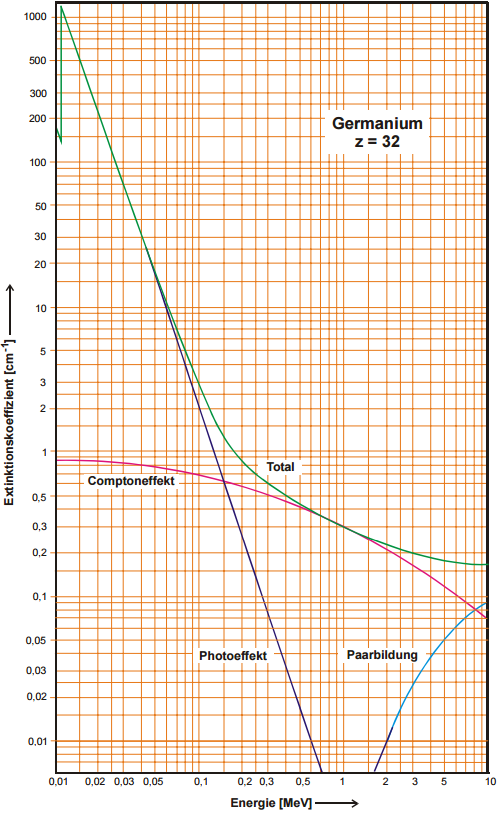
\includegraphics[height=20cm]{picture/Absorbtionskoeffizient.PNG}
	\caption{Der Absorbtionskoeffizient in Abhängigkeit der Energie am Beispiel von Germanium. \cite[7]{sample}}
	\label{fig:Absorbtionskoeffizient}
\end{figure}


\subsection{Eigenschaften von \texorpdfstring{$\beta$}{}-Strahlung}
$\beta$-Strahlung entsteht, wenn ein Neutron oder ein Proton im Atomkern zerfällt. Im folgenden wird allerdings nur die häufiger auftretende $\beta^-$-Strahlung betrachtet. Dabei zerfällt ein Neutron $n$ zu einem Proton $p$, einem Elektron $\beta^-$ und einem Antineutrino $\overline{\nu}_\text{e}$:
\begin{equation*}
	n \to p + \beta^- + \overline{\nu}_\text{e} \ .
\end{equation*}
Die dabei freiwerdende Energie ist konstant und verteilt sich kontinuierlich auf das Elektron, das Antineutrino und den Rückstoßkern. Damit kann das kontinuierliche Spektrum der $\beta$-Strahlung erklärt werden. Die Maximalenergie $E_\text{max}$, die das Elektron dabei aufnehmen kann ist die gesamte freiwerdende Energie. \\
Das $\beta$-Teilchen erleidet, beim Durchlaufen des Absorbers eine Vielzahl von Wechselwirkungen (Streuprozesse) regestriert. Dabei treten im wesentlichen drei Streuprozesse auf. \\
Bei der \textbf{Rutherford-Streuung}, erfahren die $\beta$-Teilchen eine zum Teil beträchtliche Richtungsänderung durch das Coulomb-Feld des Kerns, es treten aber nur geringe Energie verluste auf. Dadurch werden die Teilchen gestreut und die Intensität nimmt ab. Außerdem legen die Teilchen eine größere Strecke in dem Absorber zurück als nur die Dicke des Absorber. Deswegen steigt die Wahrscheinlichkeit das andere Wechselwirkungen eintreten. \\
Bei der \textbf{inelastischen Streuung am Atomkern} werden die Elektronen am Coulomb-Feld des Kerns gestreut. Dabei werden sie beschleunigt werden und beschleunigte Ladung emittiert Strahlung. Diese Strahlung heißt Bremsstrahlung, da sie dem Elektron Energie entzieht und dieses dadurch bremst. \\
Allerdings ist die wesentliche Wechselwirkung die \textbf{inelastische Steuung am Elektron} im Absorber. Die $\beta$-Teilchen treffen dabei auf Elektronen und lösen dies aus dem Atom aus bzw. regen das Atom an. Da das $\beta$-Teilchen eine sehr viel größere Energie als die Auslöseenergie der Elektronen besitzt, kann es eine Vielzahl dieser ionisierenden Prozesse durchführen. \\
Es kann nun für natürliche $\beta$-Strahler (also für $\beta^-$-Strahlung) gezeigt werden, das diese auch exponentiell abfällt. Erst für Absorberdicken, die nah an der maximalen Reichweite der Strahlung liegen, gilt dieser Verlauf nicht mehr. Nach der maximalen Reichweite $R_\text{max}$ wird nur noch die Bremsstrahlung und die Hintergrundstrahlung gemessen. Nun wird die Strahlungsintensität logarithmiert und gegen die Massenbelegung des Absorbers aufgetragen (siehe Abbildung \eqref{fig:Absorbtionskurve}). Die Massenbelegung $R$ des Absorbers lässt sich über
\begin{equation}
	R = \rho\,D
	\label{eqn:R}
\end{equation}
bestimmen.

\begin{figure}[H]
	\centering
	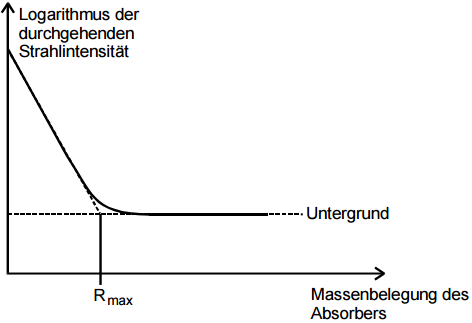
\includegraphics[height=7cm]{picture/Absorbtionskurve.PNG}
	\caption{Die Absorbtionskurve zur Bestimmung der maximalen Reichweite. \cite[12]{sample}}
	\label{fig:Absorbtionskurve}
\end{figure}

$R_\text{max}$ wird durch die Teilchen mit der höchsten Energie bestimmt, deswegen kann damit auf $E_\text{max}$ geschlossen werden.
\begin{equation}
	E_\text{max} = 1.92 \cdot \sqrt{R^2_\text{max} + 0.22 \cdot R_\text{max}}
	\label{eqn:Emax}
\end{equation}
$E_\text{max}$ wird dabei in $10^6$\,eV und $R_\text{max}$ in $\frac{\text{g}}{\text{cm}^2}$ angegeben.
























\subsection{Fehlerrechnung}
Sämtliche Fehlerrechnungen werden mit Hilfe von Python 3.4.3 durchgeführt.
\subsubsection{Mittelwert}
Der Mittelwert einer Messreihe $x_\text{1}, ... ,x_\text{n}$ lässt sich durch die Formel
\begin{equation}
	\overline{x} = \frac{1}{N} \sum_{\text{k}=1}^\text{N} x_k
	\label{eqn:ave}
\end{equation}
berechnen. Die Standardabweichung des Mittelwertes beträgt
\begin{equation}
	\Delta \overline{x} = \sqrt{ \frac{1}{N(N-1)} \sum_{\text{k}=1}^\text{N} (x_\text{k} - \overline{x})^2}
	\label{eqn:std}
\end{equation}

\subsubsection{Gauß'sche Fehlerfortpflanzung}
Wenn $x_\text{1}, ..., x_\text{n}$ fehlerbehaftete Messgrößen im weiteren Verlauf benutzt werden, wird der neue Fehler $\Delta f$ mit Hilfe der Gaußschen Fehlerfortpflanzung angegeben.
\begin{equation}
	\Delta f = \sqrt{\sum_{\text{k}=1}^\text{N} \left( \frac{ \partial f}{\partial x_\text{k}} \right) ^2 \cdot (\Delta x_\text{k})^2}
	\label{eqn:var}
\end{equation}

\subsubsection{Lineare Regression}
Die Steigung und y-Achsenabschnitt einer Ausgleichsgeraden werden gegebenfalls mittels Linearen Regression berechnet.
\begin{equation}
	y = m \cdot x + b
	\label{eqn:reg}
\end{equation}
\begin{equation}
	m = \frac{ \overline{xy} - \overline{x} \overline{y} } {\overline{x^2} - \overline{x}^2}
	\label{eqn:reg_m}
\end{equation}
\begin{equation}
	b = \frac{ \overline{x^2}\overline{y} - \overline{x} \, \overline{xy}} { \overline{x^2} - \overline{x}^2}
	\label{eqn:reg_b}
\end{equation}
